\chapter{第一格(前)}

\emoji{l_ket} 
《猫的日记》是由"悠闲的xia","大姐姐一样的mifa","稳重的yure","孩子气的feel"四个人登场的欢乐向漫画.

虽然都是Arna的大学的学生,但是由于和日本的学年制度不同,3个人都只有15岁.

今天学校来了一只白猫.

进入了Xia的教室、一边闲逛一边坐上了没有人的桌子.

这是到了休息时间,xia他们跟猫说话的场景。


●1格
\begin{figure}[H]
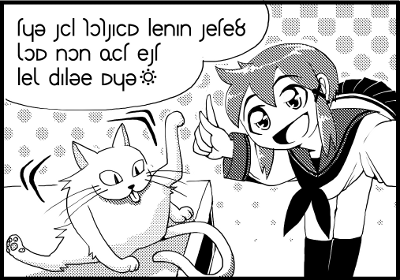
\includegraphics[width=0.5\textwidth]{ARKA/uni1.png}%或者height=\textheight
\end{figure}



\emoji{l_diina} 
这个棕毛就是"悠闲的xia".

她是从首都Arna南边的Kadish搬过来的,那是滨海的都市,是温暖的度假胜地。

Kadish人多是成熟悠闲的类型,xia也是。


\emoji{x_tisse} 
穿着日本的水手服呢.Arbazard也有这样的衣服吗?

看图同时了解文化可是一石二鸟啊.

这样说...哇,没有转写的幻字啊ーヽ(;´·ω·)ノ生幻字啊{\tiny 怕怕}

\footnote{作者注:严格来Arna大学没有制服,为了分辨角色而做了权宜.}

\emoji{l_nakx} 
先从字母转写开始吧.慢慢来.

我也算做了一些转写练习,记得可牢了。

\FiveStar 转写

xia: tyu sil koksaim lenan sete? xom non fit est lex palue myu (xante


\emoji{x_loki} 
嘿,那个数字8一样的东西是问号啊.

最后的文字是啥?工厂的地图记号吗,还是太阳....


\emoji{l_deyu} 
太阳吗?嘟嘟---.这是月亮哦,满月。

表示说话者的语调非常高兴。

满月在Arka叫xante,转写的时候就写"(xante"吧.


\emoji{x_nal} 
连表示说话方式的文字都有呢。好厉害。日语的(笑)啊,"♪"啊之类的。

不过,最初的句子是"tyu sil koksaim lenan sete?"吗。果然到正篇了吗,单词一下子就难起来了。

......咦?好像tyu和sil在理论编教过了。tyu是女用词"你",sil是表示未来形的副词。

啊啊,记忆模糊了(>\_<)。在词典查sil吧。

----

[名词]未来、将来

[纯副词]\~{}将要做.未来时的副词。

[动词]\~{}将要做。未来时的系词。

[形容词]未来的

[反意词]ses

19:制:sikt(之后)

【用例】

amir sil 未来的丈夫


----

\emoji{a_niit} 
表示未来形的副词就是sil。是纯副词方面的呢。

另外还有"未来的名词含义呢"。同时掌握不同类型的语义,感到知识增加了。

不过,"tyu sil koksaim lenan sete?"的sil视作哪一种词类比较好呢?


\emoji{x_niit} 
额......tyu不是动词,那么sil作副词的解釈就说不通了。

既然Arka是SVO,tyu应该是主语.这样sil就是动词,这是3号的语义。

呐,Lein,未来时的系词又是什么?不是,我知道未来时,只是......


\emoji{l_rana} 
系词就是be动词哟。

sil一个词就是will be的意思。


\emoji{x_lo} 
这样啊。所以意思就是"你将是\~{}"吧。

......有什么用呢,tyu sil koksaim lenan......。

啊,要是看仔细些,lenan也在理论编出来过呢。%<a href="study_mive1_10.html" 

那么.意思就成了,"你将是我们的koksaim"。


\emoji{a_pels} 
さすがにkoksaimは引かないと分からないわね。
参考までに。

\emoji{x_niit} 
同样的班......啊,就是说同班同学啊。

就是说"你将是我们的同班同学"。


\emoji{a_tia} 
这就对了!

那么问题来了。koksaim的哪个部分是"同"哪个部分是"班"呢?


\emoji{x_pels} 

等会等会......等式是koksan,同一个小组的伙伴是koksems......kok还是koks呢......。


\emoji{a_niit} 
很好的着眼点呢。那么,"同"就是"kok"。

比较上下的单词,就能加深理解,这就是词典的好处呢。


\emoji{x_lo} 
怎么说呢,这个字典连物理,地理,气象的用于都有呢......。

还有,"tyu sil koksaim lenan sete?"最后的"sete"是什么啊?

----

[文末纯词][rente]kok
古

----


\emoji{x_naki} 
啊呀,满是tag......。

诶,这是啥?


\emoji{l_asex_kal}

这个啊,"sete可归类为句末使用的纯词","sete是稳中女子所使用的词语","意义与kok相同"。

文末纯词就是日语的``\~{}ね''``\~{}さ''``\~{}だよ''``\~{}だわ''``\~{}でしょ?''这样的单词。

而后,有时间的时候、去调查一下yunk和milia吧。

先不管了,这时候应该查查kok――

----

[形容词]同じの

[反意词]koot

[格词]和\~{}相同、像\~{}一样

[文末纯词]"\~{}么?"请求确认。
[接续词]t和k都是同一类\~{}。

[数学]合同\footnote{几何变换中就有合同变换,指变换后的图形在与原图在大小和结构上都相等.}

[音乐]simile\footnote{指照前面方式演奏}

13 古:koko。纯词用法有``和我的想法相同吗?''这样的意思。

【成句】im kok 同时
【用例】

ti siina miik kok? 你喜欢苹果么?

an kok ti et kai. 我像你一样大。


----

\emoji{x_vesn} 
啊、找到"文末纯词"了。

嘿、像``\~{}么?''一样有确认的意思呢.

这么说、"tyu sil koksaim lenan sete?"是``你就是我们的同班同学么?''的意思吧。

哦这样啊。进入教室的猫住习惯了,是说的这个意思。

呼哇ーー,好不容易才弄明白了。


\emoji{l_niit} 
辛苦啦♪


\emoji{x_nal} 
谢谢ー。

好厉害的完成感啊,Lein!

好!好一部分先休息,我们来攻略第二格吧!